\chapter{Propuesta de un sistema para gestionar los Certificados Académicos}\label{chapter:proposal}

En el presente capítulo se presenta la solución que se propone para dar respuesta al problema planteado, comentando el abanico de posibilidades que existen para elegir la metodología de desarrollo de \textit{software} más adecuada a nuestro proyecto y sobre el tipo de desarrollo a seguir. Contiene la descripción de los requerimientos del sistema tanto funcionales como no funcionales. Se detallan y justifican los principales actores y se hace una descripción de los casos de usos que incluyen todo lo que el sistema debe hacer. Se describe el diseño arquitectónico, además de los patrones de diseño empleados.

%\section{Metodología de desarrollo de software adoptada}
%Las metodologías son un conjunto de procedimientos, técnicas, herramientas y ayudas a la documentación para el desarrollo de software [\cite{91}]. Guían el proceso de desarrollo de software, e imponen una disciplina sobre el desarrollo del mismo con el fin de hacerlo más predecible y eficiente.

%Existen en el mundo diferentes metodologías para llevar a cabo el desarrollo de software. Agrupadas en las conocidas metodologías pesadas o tradicionales y las metodologías ágiles [\cite{92}].

%\begin{itemize}
	%\item Metodología Tradicional: impone una disciplina de trabajo sobre el proceso de desarrollo del \textit{software}, con el fin de conseguir un sistema más eficiente. Se centra especialmente en el control del proceso, mediante una rigurosa definición de roles, actividades, artefactos, herramientas y notaciones para el modelado y documentación detallada.
	%\item Metodología Ágil: permite adaptar la forma de trabajo a las condiciones del proyecto, consiguiendo flexibilidad e inmediatez en la respuesta para adaptar el proyecto y su desarrollo a las circunstancias específicas del entorno.
%\end{itemize}


%Tras revisar el abanico de posibilidades metodológicas, y dadas las características del proyecto, del equipo de desarrollo y el poco tiempo disponible, se ha decidido adaptar la metodología Scrum.

%Scrum es una metodología ágil donde se fomenta el trabajo en equipo y entregas continuas con el objetivo de ser altamente productivos [\cite{92}]. Esta metodología incluye distintos roles:
%\begin{itemize}
	%\item \textit{Product Owner}: Representa la voz del cliente, deben de entender las necesidades de estos y encargarse de comunicar el objetivo del proyecto, negociar con el equipo de desarrollo las tareas que realizarán y además dar una opinión acerca de los entregables en cada iteración.
	%\item \textit{Scrum Master}: Es el encargado del cumplimiento de las reglas de la metodología Scrum, ayudando y fomentando el trabajo en equipo. El \textit{Scrum Master} programa y dirige las reuniones del equipo, asegurando que se cumplen las reglas de estas. Por último, elimina cualquier bloqueo o impedimento que pueda tener el equipo.
	%\item Equipo de desarrollo: Es el encargado de desarrollar las tareas que se encuentran programadas en el sprint, realizar las estimaciones de tiempo de estas, negociar con el \textit{product owner}, y completar las entregas del producto.
%\end{itemize}

%Este tipo de metodología trata de realizar entregas del producto final, fijadas en un acuerdo entre el equipo de desarrollo y el \textit{product owner}, para conseguir un resultado completo con cada iteración. Normalmente las iteraciones son de 2 semanas, aunque puede haber equipos que prefieren 3 o 4 semanas.

%El \textit{backlog} es un almacén en el cual se encuentran las tareas a realizar, ordenadas por prioridad [\cite{93}]. El equipo de desarrollo es el encargado de añadir y realizar las estimaciones de las tareas, siendo el \textit{product owner} el responsable de priorizar estas. Una vez las tareas se encuentran priorizadas de mayor a menor importancia, según la capacidad del equipo de desarrollo, estos proceden a crear el \textit{sprint}. El \textit{sprint} es el período de tiempo determinado para realizar el trabajo acordado para alcanzar los objetivos propuestos. Es muy importante tener bien definida la tarea, junto con las pruebas de aceptación y una estimación en horas o puntos.

%Antes de comenzar un \textit{sprint}, se realiza la reunión llamada \textit{sprint planning}, para seleccionar y comunicar qué tareas es capaz de realizar el equipo, las cuales son seleccionadas del inicio del \textit{backlog}. Una vez finalizado el \textit{sprint} el \textit{product owner} realiza una revisión del trabajo entregado por el equipo de desarrollo y una reunión de retrospectiva en la cual todos los integrantes dejan sus impresiones con el objetivo de mejorar como equipo.

\section{Análisis del Sistema}

\subsection{Actores del sistema}
Los actores representan entidades que interactúan con el sistema, un actor del sistema es aquel que se beneficia de los resultados de las funcionalidades del mismo [\cite{91}]. 

Se definen dos tipos de usuarios principales que pueden interactuar con la plataforma: \textbf{anónimos} y \textbf{gestores}. El usuario \textbf{anónimo} es un \textbf{usuario público} que puede acceder sin registrarse a las funcionalidades públicas del sistema.

Los \textbf{gestores} serán usuarios registrados en una base de datos conocida por el sistema. Estos usuarios tendrán acceso a una sección de \textit{back office} que le permitirá realizar tareas de gestión en la plataforma. Además, contarán con un rol definido en dicho sistema de terceros cuyo rol viajará en la respuesta de autenticación del mismo al nodo cliente (borde del \textit{backend} de la solución a implementar).

\subsection{Casos de uso del sistema}
La forma en que los actores utilizan el sistema es representada a través de los casos de usos [\cite{91}]. Estos últimos son artefactos narrativos que describen, bajo la forma de acciones y reacciones, el comportamiento del sistema desde el punto de vista del actor.

%Los casos de usos identificados en el presente trabajo son enunciados a continuación:
\begin{figure}[!h]
	\centering
	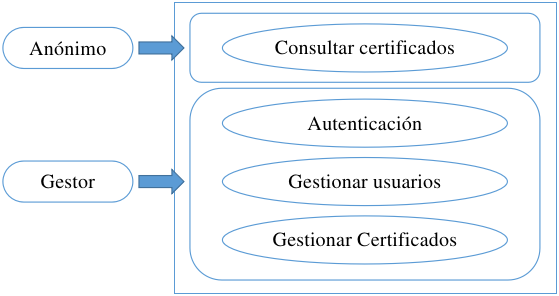
\includegraphics[width=\linewidth]{Graphics/caso-uso.png}
	\caption{Diagrama de casos de uso del sistema}
	\label{fig:11}
\end{figure}

En la Figura \ref{fig:11} se observa el diagrama de casos de uso del sistema a que se presenta. Los diagramas de casos de usos [\cite{91}] son un tipo de diagrama dónde se puede representar el comportamiento esperado del sistema, desde la visión de los usuarios, sin llegar a un alto nivel de especificación acerca de cómo se implementan las acciones. 

Los principales elementos que nos encontramos en él son:
\begin{itemize}
	\item Sistema: Representa con un rectángulo los límites del sistema, los actores se ubican fuera de la figura.
	\item Caso de uso: Representado con un óvalo y un texto identificativo, identifican una determinada acción.
	\item Actor: Son las entidades externas al sistema que interactúan con él.
\end{itemize}

Las acciones: gestionar certificados y gestionar usuarios se dividen a su vez un subacciones. Es necesario sobre estos modelos poder crear nuevas entradas y eliminar, editar o invalidar las existentes. En el caso de los certificados es necesario además un proceso de validación por tres usuarios gestores con roles específicos.

%\subsubsection{Descripción de los casos de uso del sistema}
En las tablas \ref{tab:CU1} y \ref{tab:CU2} se exponen dos de los casos de uso de alto nivel, para lograr entender los procesos globales de la aplicación. El resto puede ser encontrado en los anexos \ref{appendix:useCase}.

\begin{table}[!h]
	\begin{center}
		\begin{tabular}{|c|p{10cm}|}
			\hline \textbf{CU1} & Validar certificados \\ 
			\hline \textbf{Actor} & Gestor \\ 
			\hline \textbf{Descripción} & Ciertos usuarios de tipo gestor podrán validar los títulos asociados a una persona al introducir el identificador que representa al certificado.  \\ 
			\hline 
		\end{tabular}
		\caption{Caso de uso: Validar Certificado}
		\label{tab:CU1}
	\end{center}
\end{table}

\begin{table}[!h]
	\begin{center}
		\begin{tabular}{|c|p{10cm}|}
			\hline \textbf{CU2} & Autenticación \\ 
			\hline \textbf{Actor} & Gestor\\ 
			\hline \textbf{Descripción} & El usuario de tipo gestor deberá insertar sus credenciales (nombre de usuario y contraseña) para poder acceder al sistema.\\ 
			\hline 
		\end{tabular}
		\caption{Caso de uso: Autenticación}
		\label{tab:CU2}
	\end{center}
\end{table}

\subsection{Historias de usuario}
Las historias de usuario se usan, en el contexto de la ingeniería de requisitos ágil, como una herramienta de comunicación que combina las fortalezas de ambos medios: escrito y verbal. Describen, en una o dos frases, una funcionalidad de \textit{software} desde el punto de vista del usuario, con el lenguaje que éste emplearía. Se enfocan en qué necesidades o problemas soluciona lo que se va a construir.

Las tablas \ref{tab:HU1}, \ref{tab:HU2}, \ref{tab:HU3} se exponen algunos de las historias de uso de alto nivel, el resto pueden ser encontradas en los anexos \ref{appendix:useHistory}.

\begin{table}[!h]
	\begin{center}
		\begin{tabular}{|c|p{10cm}|}
			\hline \textbf{H.U-1} & Conocer títulos \\ 
			\hline \textbf{Usuario} & Anónimo\\ 
			\hline \textbf{Descripción} & Como usuario anónimo quiero poder conocer los certificados de una persona para poder observar las habilidades y estudios de esa persona. \\ 
			\hline 
		\end{tabular}
		\caption{Historia de Usuario: Conocer títulos}
		\label{tab:HU1}
	\end{center}
\end{table}

\begin{table}[!h]
	\begin{center}
		\begin{tabular}{|c|p{10cm}|}
			\hline \textbf{H.U-2} & Autentificación \\ 
			\hline \textbf{Usuario} & Gestor \\ 
			\hline \textbf{Descripción} & Como usuario gestor quiero poder autenticarme para poder tener acceso al sistema. \\ 
			\hline 
		\end{tabular}
		\caption{Historia de Usuario: Autentificación}
		\label{tab:HU2}
	\end{center}
\end{table}

\begin{table}[!h]
	\begin{center}
		\begin{tabular}{|c|p{10cm}|}
			\hline \textbf{H.U-3} & Cerrar sesión \\ 
			\hline \textbf{Usuario} & Gestor \\ 
			\hline \textbf{Descripción} & Como usuario gestor quiero poder cerrar la sesión actual para poder salir de forma segura del sistema. \\ 
			\hline 
		\end{tabular}
		\caption{Historia de Usuario: Cerrar sesión}
		\label{tab:HU3}
	\end{center}
\end{table}

%\subsection{Planificación de desarrollo}
%Siendo el equipo solamente una persona (el autor de este trabajo), no existe ningún rol, pero se mantiene la creación y el mantenimiento del \textit{backlog}, siguiendo una organización de \textit{sprints}, permitiendo tener alguna parte del sistema funcionando después de cada iteración, para que esto pudiera ser presentado y discutido con el cliente. Si el equipo aumentara en un futuro, se comenzaría a hacer uso de los roles definidos en la metodología.

%La fecha final del proyecto será acorde a la fecha límite de entrega de la convocatoria ordinaria del Trabajo de Fin de Grado. Por tanto, se ha establecido la duración de los sprints en 2 semanas, teniendo cada uno una carga de 34h aproximadamente por \textit{sprint}. En la tabla \ref{tab:sprints} puede verse una planificación inicial. Esta planificación es susceptible a cambios, así como la fecha de finalización podría ser cambiada.

%\begin{table}[!h]
	%\begin{center}
		%\begin{tabular}{|c|c|c|c|}
			%\hline \textbf{Sprint} & \textbf{Comienzo} & \textbf{Final} & \textbf{H.U a desarrollar} \\ 
			%\hline Sprint 0 & 3/09/2022  & 18/09/2022 & -\\ 
			%\hline Sprint 1 & 18/09/2022 & 2/09/2022 & H.U-1\\ 
			%\hline Sprint 2 & 2/09/2022 & 16/10/2022 & H.U-2, H.U-3\\ 
			%\hline Sprint 3 & 16/10/2022 & 30/10/2022 & H.U-4\\ 
			%\hline Sprint 4 & 30/10/2022 & 14/11/2022 & H.U-5, H.U-6, H.U-7\\ 
			%\hline Sprint 5 & 14/09/2022 & 25/10/2022 & H.U-8\\ 
			%\hline 
		%\end{tabular}
		%\caption{\textit{Backlog} inicial}
		%\label{tab:sprints}
	%\end{center}
%\end{table}

\section{Diseño del sistema}
En esta sección se describe cómo está ideado el sistema, pasando por su arquitectura, los patrones usados, los roles que tienen los usuarios y los datos que representan un certificado académico. Se puntualizarán también elementos de seguridad y será presentado el diagrama de despliegue del sistema.

\subsection{Arquitectura del sistema}
La arquitectura de un \textit{software} se encarga de entender cómo debe organizarse el sistema y cómo tiene que diseñarse la estructura global del mismo [\cite{91}]. Constituye el enlace crucial entre el diseño y la ingeniería de requisitos, ya que identifica los principales componentes estructurales en un sistema y la relación entre ellos. La salida del proceso de diseño arquitectónico consiste en un modelo arquitectónico que describe la  forma en que se organiza el sistema como un conjunto de componentes en comunicación. La arquitectura de \textit{software} representa un elemento fundamental pues afecta el desempeño del sistema, así como su capacidad de distribución y mantenimiento.

Según [\cite{99}], la arquitectura de un sistema puede basarse en un patrón o un estilo arquitectónico particular. Un patrón arquitectónico es una descripción de una organización del sistema, captan la esencia de una arquitectura usada en diferentes sistemas de \textit{software}.

Para este sistema se ha optado por dividirlo en dos niveles: lógica de negocio y persistencia (Figura \ref{fig:8}). 

\begin{figure}[h]
	\centering
	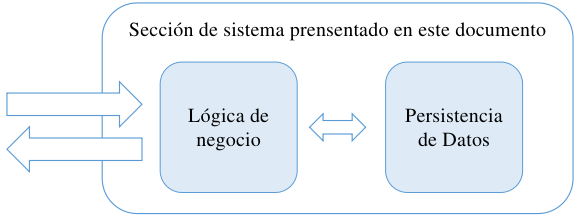
\includegraphics[width=\linewidth]{Graphics/arquitectura-bs.png}
	\caption{Arquitectura del sistema}
	\label{fig:8}
\end{figure}

El nivel de negocio es el encargado de facilitar al nivel de presentación los datos necesarios, a la vez que recolecta los datos aportados por este para procesarlos. Este nivel está conectado con el nivel de persistencia, enviándole peticiones para almacenar o recuperar datos de este [\cite{96}].

El nivel de persistencia es donde residen los datos y generalmente está formada por un gestor encargado de realizar el almacenamiento de datos. Este nivel recibe las peticiones de negocio, quien le dice qué datos necesita o qué datos tiene que almacenar [\cite{96}]. 

La persistencia de datos se divide en dos componentes: el almacenamiento de los usuarios y el de los certificados. Para almacenar los usuarios se escogió una base de datos relacional PostgreSQL, mientras que para almacenar los certificados se ha usado tecnología blockchain con el software Hyperledger Fabric. Ambas componentes son gestionadas por el nivel de negocio y entre ellas (Usuarios y Certificados) no tienen comunicación directa (Figura \ref{fig:9}).

\begin{figure}[h]
	\centering
	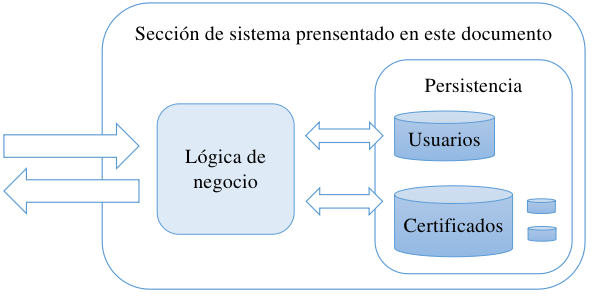
\includegraphics[width=\linewidth]{Graphics/arquitectura-ex.png}
	\caption{Arquitectura del sistema expandida}
	\label{fig:9}
\end{figure}

Durante el capítulo de Estado del Arte se explicó la razón de usar Go. Dado que esta capa lógica tiene que aceptar peticiones generadas por el nivel de presentación y marcar un límite bien definido entre ambas, se usa la biblioteca `Iris GO'. Iris Go es un web framework que permite crear los endpoints necesarios para un desacople limpio y poder afirmar que el sistema propuesto sigue una arquitectura cliente-servidor.

\subsection{Patrones de diseño seguidos}

La arquitectura es necesaria para comprender el sistema, organizar el desarrollo, fomentar la reutilización y hacer evolucionar el sistema. Para definirla es muy importante tener en cuenta un patrón de diseño o modelo de abstracción que nos sirva para poder estructurar de manera eficaz todos los componentes de la aplicación.

\subsubsection{Patrones GRASP}
Los patrones GRASP (Patrones Generales de Software para Asignación de Responsabilidades) describen los principios fundamentales de diseño de objetos para la asignación de responsabilidades. Las responsabilidades  están relacionadas con las obligaciones de un objeto en cuanto a su comportamiento [\cite{97}]. Entre los patrones GRASP empleados en la presente propuesta se encuentran:

\begin{itemize}
    \item Controlador: El patrón controlador es un patrón que sirve como intermediario entre una determinada interfaz y el algoritmo que la implementa. 

	Se dividen las distintas funcionalidades del sistema en endpoints que sean especializados y no genéricos. Cada uno de estos endpoints serán los encargados de utilizar los servicios que son los que saben como construir la respuesta. Con esta cantidad de endpoints se aumenta la cohesión y disminuye el acoplamiento.
	
	\item Bajo Acoplamiento: El acoplamiento es una medida de la fuerza con que una clase está conectada a otras clases, con que las conoce y recurre a ellas. El bajo acoplamiento soporta un diseño de clases más independientes, que reducen el impacto de cambios, y permite que sean más reutilizables.
	
	La capa de negocio implementada en go y basada en paquetes permite un bajo acoplamiento entre sus componentes. Estos pueden ser creados, modificados o eliminados en cualquier momento, lo que proporciona que la dependencia entre ellos sea baja.
	
	\item Alta Cohesión: La cohesión es una medida de la fuerza con la que se relacionan las clases y el grado de focalización de las responsabilidades de un elemento. Cada elemento del diseño debe realizar una labor única dentro del sistema, no desempeñada por el resto de los elementos, y auto-identificable. Una clase con baja cohesión realiza muchas labores no relacionadas o realiza demasiado trabajo.
	
	La capa de negocio implementada en go y basada en paquetes permite la organización del trabajo en cuanto a la estructura del proyecto y la asignación de responsabilidades con una alta cohesión. Cada componente realiza solo las funcionalidades para las cuales fueron creados, colaborando entre ellos para cumplir con el resto de las funcionalidades, generando un bajo acoplamiento y fomentando la reutilización. Esto hace posible que el sistema sea flexible a cambios sustanciales con efecto mínimo
\end{itemize}

\subsubsection{Patrones GoF}
Los patrones GoF(Gang of Four) utilizados en la propuesta de solución son los siguientes:

\begin{itemize}
	\item Bridge (Puente): Desacopla una abstracción de su implementación.
	
	El nivel de negocio tiene capas internas. Una de estas capas es la encargada de comunicarse con los framework que tratan la persistencia. De esta forma cuando un dato es requerido se le pide a esa capa, abstrayéndose de como es buscado. Esta capa sirve de puente entre ambos niveles: negocio y persistencia
	
	\item Command (Orden): Este patrón encapsula una operación en un objeto, permitiendo ejecutar dicha operación sin necesidad de conocer el contenido de la misma.
	
	El Proceso de validación de certificados sigue este patrón, Aún sin conocer el tipo de validador que sea
	el usuario este puede emitir la validación. El sistema se encargará luego de entender el proceso y modificar los campos pertinentes del certificado.	
\end{itemize}

\subsection{Roles de usuarios}

El proyecto consta con varios roles que tienen distintas funcionalidades. El personal de las instituciones universitarias podrán realizar consultas más especializadas y gestionar los certificados digitales según el rol que posea, para ello necesitarán iniciar sesión con sus credenciales asignadas. Los roles que se manejarán para los usuarios gestores son los siguientes:

\begin{itemize}
	\item \textbf{Administrador de Sistemas}: Encargado de manejar los usuarios que participan en el sistema: crearlos, editarlos, eliminarlos o invalidarle sus credenciales.
	\item \textbf{Administrador de Certificados}: Usuario que tiene los permisos para gestionar los certificados: crearlos, editarlos, eliminarlos o invalidarlos. Este rol no valida los certificados.
	\item \textbf{Secretario General}: Usuario que tiene los permisos para validar certificados recién creados. Puede invalidar los certificados que encuentre inconsistentes.
	\item \textbf{Decano de Facultad}: Usuario que tiene los permisos para validar certificados aprobados por el Secretario General. Puede invalidar los certificados que encuentre inconsistentes.
	\item \textbf{Rector de Universidad}: Usuario que tiene los permisos para validar certificados aprobados por el decano. Es el último eslabón para hacer un certificado válido. Puede invalidar los certificados que encuentre inconsistentes.
	\item \textbf{Inválido}: Usuario al que le fueron retirados sus privilegios por un administrador de sistema.
\end{itemize}

\subsection{Estructura de los certificados}
El sistema que se presenta no registrará binarios (copia digital de título, entre otras), sino que los certificados serán representados por propiedades:
\begin{itemize}
	\item \textbf{ID}: El identificador de los certificados es con fines de facilitar su búsqueda. No tiene una representación real en un certificado a papel. El campo es generado utilizando la fecha y hora de creación de la credencial. Su estructura es: YYYYMMDDHHMMSS (año, mes, día, hora, minuto y segundo concatenados)
	\item \textbf{Certificación}: Título que se le otorga al acreditado.
	\item \textbf{Título de oro}: Campo que representa si se alcanzó la distinción.
	\item \textbf{Emisor}: Centro que emite el certificado. Ej: Universidad de la Habana.
	\item \textbf{Acreditado}: Persona a la que se emite el título.
	\item \textbf{Fecha}: Fecha de emisión del documento.
	\item \textbf{Creador}: Usuario que creó dicho certificado en la base de datos.
	\item \textbf{Secretario, Decano y Rector}: Tres propiedades que guardan los nombres de los funcionarios que validan la Credencial.
	\item \textbf{Tomo y folio de facultad y universidad}: Dos propiedades que almacenan Tomo y folio bajo el cual fueron inscritos los documentos tanto en la facultad como en la universidad
	\item \textbf{Estado}: Refleja el estado actual del documento.
	\item \textbf{Razón de Invalidación}: Refleja, de estar el certificado en estado invalidado, la razón de la decisión.
\end{itemize}

Los certificados pueden tener cinco estados:
\begin{itemize}
	\item \textbf{Inválido}: El certificado fue invalidado por un usuario gestor con los permisos adecuados.
	\item \textbf{Creado}: El documento fue creado, pero no posee ninguna firma de validación.
	\item \textbf{Firmado por Secretario}: El documento fue validado por un usuario gestor con rol de `secretario'.
	\item \textbf{Firmado por Secretario y Decano}: El documento fue validado por un usuarios gestores con rol `secretario' y `decano'.
	\item \textbf{Válido}: El certificado fue validado por usuarios gestores con rol `secretario', `decano' y `rector'.
\end{itemize}

Los certificados tiene que pasar por varios estados en secuencia antes de tener el estado `Válido' [\ref{fig:12}]
\begin{figure}[h]
	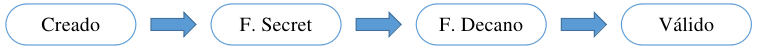
\includegraphics[width=\linewidth]{Graphics/status.png}
	\caption{Proceso de certificados hasta el estado de Válido}
	\label{fig:12}
\end{figure} 

\subsection{Elementos de seguridad}
La autenticación de portador (también llamada autenticación de token) es un esquema de autenticación HTTP que involucra tokens de seguridad llamados \textit{Bearer tokens} [\cite{98}]. El nombre ``Autenticación de portador'' puede entenderse como ``dar acceso al portador de este token''. El \textit{Bearer token} es una cadena críptica, generalmente generada por el servidor en respuesta a una solicitud de inicio de sesión. Este inicio de sesión es necesario para los gestores: actores del sistema que dependiendo de su rol tiene la capacidad de modificar los datos almacenados en la capa de persistencia. 
%Como habíamos mencionado previamente en la definición de actores del sistema, los gestores son usuarios registrados en un sistema de terceros y además cuentan con un rol definido en dicho sistema de terceros. Nuestra interfaz de usuario debe ser capaz de mostrar visualmente las secciones del \textit{back office} relacionadas a los permisos asociados al rol del usuario autenticado.

La solución propuesta en este trabajo creará y verificará tokens de identificación (\textit{Bearer token}) para cada usuario. Estos tokens serán entregados a la capa que se comunique con los endpoints, la cual enviará sus peticiones con estos tokens como muestra de la identidad. Codificado en estos está la información del nombre del usuario y su rol en el sistema. Cada endpoint, si así lo requiere, podrá consultar esos datos y controlar el acceso a esas funcionalidades.

Para evitar la autenticación de clientes mal intencionados que pretendan comprometer la seguridad de la base de datos donde se almacenan los usuarios; se guardará un hash de las contraseña en lugar de la contraseña misma. Como se sabe, por las cualidades de las funciones hash, conociendo el hash no se puede obtener la contraseña a partir de la cual se generó.

Para mantener la integridad de los datos almacenados en el nivel de persistencia se harán comprobaciones de validación. Estas comprobaciones serán realizadas si una operación que implique modificación de datos puede crear inconsistencia en estos. Un ejemplo del proceso está en la edición de certificados. El estado de un certificado representa los directivos que faltan por validarlo (o en casos particulares si está invalidado), una vez lleguen los nuevos valores de la edición se comprobará que en el certificado no falte ninguno de los validadores que su estado refleja ya han firmado.

\subsection{Diagrama de despliegue}
Un modelo de despliegue consiste en una representación estructural de la arquitectura del sistema desde el punto de vista de la distribución de los artefactos del software en los destinos de despliegue; definiendo a los artefactos como representaciones de elementos concretos en el mundo físico que son el resultado de un proceso de desarrollo [\cite{91}]. La Figura \ref{fig:10} representa el diagrama de despliegue del sistema que se propone.

\begin{figure}[h]
	\centering
	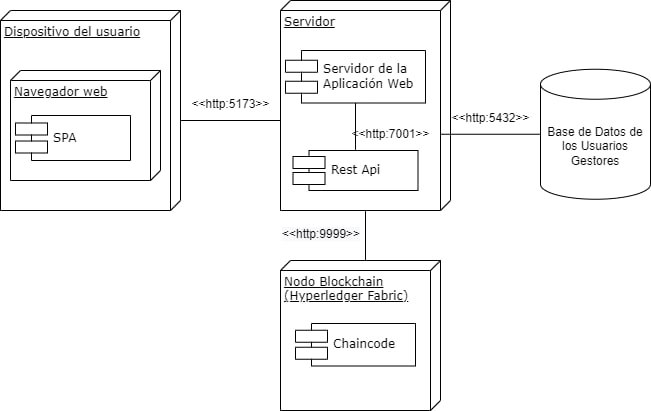
\includegraphics[width=\linewidth]{Graphics/diagrama.png}
	\caption{Diagrama de despliegue del sistema.}
	\label{fig:10}
\end{figure}

